\documentclass[a4paper,12pt,english, T1]{book}
\usepackage[utf8]{inputenc}
\usepackage[T1]{fontenc}
\usepackage{tikz-dependency}
\usepackage{times}
\usepackage{multirow}
\usepackage{tablefootnote}
\usepackage{booktabs}
\usepackage{covington}
\usepackage{relsize}
\usepackage{hyperref}
\usepackage{appendix}
\usepackage{duomasterforside}
\usepackage{emptypage}
\usepackage{tocbibind}
\usepackage{url}
\usepackage{tikz}
\usepackage{apacite}
\usepackage{amsmath}

\usepackage{fancyhdr}
\pagestyle{fancy}
\fancyhf{}
\renewcommand{\sectionmark}[1]{\markright{\thesection.\ #1}}
\renewcommand{\chaptermark}[1]{\markboth{\textsc{\thechapter.\ #1}}{}}
\lhead[\leftmark]{}
\rhead[]{\rightmark}
\lfoot[\thepage]{}
\rfoot[]{\thepage}

\title{Improving Frame Accuracy for Semantic Dependency Parsing}
\author{Arash Saidi}

\begin{document}
\duoforside{}

\chapter*{Abstract}
\thispagestyle{empty}

This thesis presents an in-depth contrastive error analysis of a set of semantic dependency parsing systems. Based on the empirical results of our analysis we found semantic frame classification to be an interesting case study. As part of this thesis we have made a semantic frame classifier that outperforms previous results. The semantic frame classifier is the result of rigorous experimentation with four set of features: (1) lexical, (2) morphological, (3) syntactic, and (4) semantic. We show that our results outperform previous results. We also show that our classifier can be used to extend and improve the frame semantic classification accuracy of two existing state-of-the-art semantic dependency parsing systems.

% the results of frame classification of two existing state-of-the-art semantic dependency parsing systems.

% This thesis presents a systematic, empirical investigation of how an existing PoS tag set can be modified and optimized for the task of syntactic dependency parsing of Norwegian. The tag set of the Norwegian Dependency Treebank is modified and optimized through experiments with the morphological features in the treebank. The experiments are complemented by evaluation of a range of state-of- the-art PoS taggers and syntactic parsers applied to Norwegian. The results of our work are concrete contributions to the Norwegian NLP community: (i) a data set split (training/development/test) of the Norwegian Dependency Treebank; (ii) a PoS tag set optimized for syntactic dependency parsing of Norwegian; (iii) a PoS tagger model trained on the treebank; and (iv) a syntactic parser model trained on the treebank.
\chapter*{Acknowledgements}
\thispagestyle{empty}

This thesis is submitted for the degree of Master of Science at the University of Oslo. My supervisors have been Stephan Oepen and Lilja Øvrelid. I am thankful for their insights, helpful advice and patience.

I want to thank my good friend, fellow student, and co-worker Petter Hohle for proofreading and being a great motivator. I want to thank my co-worker Anna Therese Hägg for proofreading. I thank my girlfriend Marit for encouragement, love and support.

\frontmatter{}
\fancyhead[LE]{\nouppercase\leftmark}
\fancyhead[RO]{\nouppercase\rightmark}
\tableofcontents{}
\listoftables{}
\listoffigures{}

\mainmatter{}
\chapter{Introduction}
\label{chap:introduction}

% Motivere hva som er resultatet, hva har jeg gjort, og hvem som trenger det, hvilken spørsmål har du stilt.

Semantic dependency parsing is a Natural Language Processing (NLP) task that aims at producing meaning representations at the sentence-level. We can state the aims of semantic dependency parsing as a way of expressing predicate-argument relations in order to answer the question of \textit{Who did What to Whom?} In this regard there is certainly an overlap between semantic dependency parsing  and \textit{semantic role labeling} (SRL). 

The task of SRL is concerned with detecting the arguments of a predicate in a given sentence. Semantic dependency parsing usually has a broader scope than argument detection. In addition to the goals of SRL, semantic dependency parsing attempts to identify various semantic phenomena, such as negation, topicalization, relative clauses, and other scopal dependencies that are not part of the scope of SRL.

Examining the research community and the publications in the field of dependency parsing, we can see a growing interest in semantic dependency parsing in recent years. This can be attributed to both the advances made in the accuracy of state-of-the-art parsers, but also due to the successful application of such parsers and their representations in a wide range of computational tasks such as Information Extraction, Textual Inference, Machine Translation, Semantic Search, and Sentiment Analysis. A set of so-called shared tasks on semantic dependency parsing, which we will present in this thesis, have also stimulated the research community towards more research on this specific type of dependency parsing.

In this thesis we present our contribution to the field of semantic dependency parsing by doing a high-level contrastive error analysis of various state-of-the-art semantic dependency parsing systems. We will closely examine their results, and compare them in order to gain insights into the areas with the potential of improvements in parsing accuracy. We will show that the error analysis provided us with the grounds for examining the so-called frames, also referred to as sense distinctions, in order to make an attempt at improving previous results. Based on this analysis we build our own pipeline for classifying semantic frames. These frames are added as an extra layer to the graph annotations of semantic dependencies. So in this sense they are not part of the semantic dependency graph itself, but acts as additional semantic information. The classification of the frames themselves rely on the semantic dependency graph as features for training the classifier.

\section{Overview} 

% Background
\paragraph{Chapter 2} provides a background for our thesis. In this chapter we briefly outline dependency grammar, and then examine various approaches to dependency based parsing. We differentiate between grammar- and data-driven dependency parsing, and formally describe both of these approaches to dependency parsing. We divide data-driven dependency parsing in two main classes: transition-based and graph-based models. We examine these two models and give examples of their implementation by presenting a few examples of tools that are openly available. Finally, we define semantic dependency parsing, and show how this approach differentiates from syntactic dependency parsing. We will also argue why we should focus on semantic dependency parsing, and provide arguments for the reasoning behind writing this thesis.

\paragraph{Chapter 3} examines a few selected state-of-the-art semantic dependency parsers. We have chosen to focus on a set of data-driven parsers that where part of the Task 18 at SemEval 2015 on \textit{Broad-Coverage Semantic Dependency Parsing} (SemEval-2015) \cite{Oepen:15}. We present the parsing systems that where part of this task, and provide the reader with a background to the technology that drives them. We will also examine the target representations used for training and testing. Here we also examine Task 8 at SemEval 2014 (SemEval-2014) (see \citeA{Oepen:14}, in order to provide the reader with more background to SemEval 2015, and the changes from one year to the next.

\paragraph{Chapter 4} builds on the previous chapter by examining the results submitted by a set of parsing systems to SemEval-2015. By way of an in-depth contrastive error analysis of a set of state-of-the-art parsers we gain insights into some common errors that these parsers share. We examine four factors of semantic dependency parsing: (1) length factors, (2) graph factors, and (3) linguistic factors and (4) frames accuracy. The insights from this chapter lay the empirical foundation for our own classification task.

\paragraph{Chapter 5} examines our own pipeline for classifying semantic frames. The analysis in Chapter \ref{chap:semantic} led us in choosing semantic frames as the focal point of our own work. In this chapter we build a pipeline for classifying semantic frames by examining a set of machine learning algorithms. We start off by presenting a baseline accuracy, and see if we can improve upon this baseline by fine tuning the machine learning algorithms, and by way of exploring a set of features used for training. We show that by using a wide range of features for our classifier, we can achieve state-of-the-art results in predicting semantic frames.

\paragraph{Chapter 6} is a summary and conclusion of our thesis. Here we give a short overview of what we have achieved in our thesis, and discuss how this relates to the research on semantic dependency parsing at large. We also discuss the possibilities for future work that might benefit from the analysis and classification task performed in our thesis.
\chapter{Background}
\label{chap:background}

This chapter provides and introduction to Dependency Grammar and Dependency
Parsing and the technical aspects ranging from the early development to state-of-the-art
dependency parsing techniques. 
\chapter{Semantic Dependency Parsing with Frames}
\label{chap:parsing}
\chapter{In-depth Contrastive Error Analysis}
\label{chap:analysis}

% Length
% Graph factors
% Linguistic factors

% Peking: Ensemble method, combination of transition-based and graph-based
% Turku: Support Vector Machines
% Lisbon: A graph algorithm


In this chapter we present an in-depth contrastive error analysis of the results of SemEval-2015 for the Peking, Turku and Lisbon systems described in Chapter \ref{chap:semantic}. As mentioned in the previous chapter, there where 6 submissions to SemEval-2015, including an `in-official' submission by a sub-set of the task organizers. We have made the choice of focusing on three of these parsing systems in our analysis. This is based on three criteria:

\begin{enumerate}
    \item The chosen systems have the highest overall scores in SemEval-2015.
    \item The technical approach of the three parsing systems are different from one another: both the local transition-based and global graph-based models that we examined in Chapter \ref{chap:background} are represented.
    \item When choosing between submissions where similar technical approach has been used, we exclude the system with the overall lower accuracy score.
\end{enumerate}

The aim of our in-depth contrastive error analysis is to gain insight into the state-of-the-art in semantic dependency parsing. We perform our study in order to:

\begin{enumerate}
    \item Find similarities and differences in the results among a chosen set of parsing systems in order to compare and contrast their strengths and weaknesses.
    \item Empirically identify and verify which types of errors that can be the focus of future research on improving the accuracy of the state-of-the-art in semantic dependency parsing.
    \item Examine whether an ensemble method based on the strengths of different parsing systems is possible in order to improve upon existing systems.
\end{enumerate}

% We will argue that the analysis presented in this chapter can highlight the correlation between the specific types of errors that these parsers make and their theoretical foundation. The analysis presented is thus based on the general knowledge of the parsing systems, as described in Chapter \ref{chap:semantic}, and the specific observations made in our analysis of their results from SemEval-2015.

In our analysis we draw inspiration from three similar studies performed by \citeA{McD:Niv:07}, \citeA{McD:Niv:11}, and \citeA{Choi:Tetreaul:Stent:15}. In these studies a comparative analysis of a set of syntactic parsers is presented where various types of errors are highlighted. The first and second study focus on three types of errors: (1) length factors, (2) graph factors, and (3) linguistic factors. The third study, in addition to these three factors, also examine the speed of parsers. We will structure our analysis in a similar fashion, but exclude speed, and include a fourth type error analysis where we examine the multi-classification task of frame predication.

In addition to narrowing down the scope in terms of choosing three parsing systems, we also exclude results for the PAS target representation. The reasoning behind this is that the DM and PAS target representations are relatively similar. Examining Table \ref{fig:data} in Chapter \ref{chap:semantic}, we observe that DM and PAS are close to identical in the number of labels, percentage of graphs being trees, and percentage of dependencies being projective. The major difference between the two target representations is the percentage of so-called singletons, i.e. nodes outside the graph. The DM target representation has approximately 5 times as many singletons as PAS. With the exception of singletons, we assume that our analysis of the DM results will yield similar results as PAS. This hypothesis was confirmed when running our parts of our analysis on PAS.

However, before we embark on our in-depth contrastive error analysis, we recap overall statistics on the three parsing systems that are the basis for our analysis.

\section{Overall Accuracy}

\begin{table}
    \centering
    \begin{tabular}{@{}cccccccccc@{}}
        \toprule
        \multicolumn{1}{c}{ }
        & \multicolumn{1}{c}{ }
        & \multicolumn{4}{c}{\textbf{DM}}
        & \multicolumn{4}{c}{\textbf{PSD}} \\
        \cmidrule(lr){3-6}
        \cmidrule(lr){7-10}
        &
        LF.av &
        LF & LP & LR & FF &
        LF & LP & LR & FF \\
        \midrule
        Peking & 85.33 & 89.09 & 90.93 & 87.32 & 63.08 & 75.66 & 78.60 & 72.93 & 49.95 \\
        Lisbon & 85.15 & 88.21 & 89.84 & 86.64 & 00.15 & 76.36 & 78.62 & 74.23 & 00.03 \\
        Lisbon* & 86.23 & 89.44 & 90.52 & 88.39 & 00.20 & 77.58 & 79.88 & 75.41 & 00.06 \\
        Turku* & 83.47 & 86.17 & 87.80 & 84.60 & 54.67 & 73.63 & 76.10 & 71.32 & 53.20 \\
        \bottomrule
        
        \\
        \toprule
        \multicolumn{1}{c}{ }
        & \multicolumn{1}{c}{ }
        & \multicolumn{4}{c}{\textbf{DM}}
        & \multicolumn{4}{c}{\textbf{PSD}} \\
        \cmidrule(lr){3-6}
        \cmidrule(lr){7-10}
        &
        LF.av &
        LF & LP & LR & FF &
        LF & LP & LR & FF \\
        \midrule
        Lisbon & 81.15 & 81.75 & 84.81 & 78.90 & 00.27 & 74.82 & 78.68 & 71.31 & 02.09 \\
        Peking & 80.78 & 81.84 & 84.29 & 79.53 & 47.49 & 73.28 & 77.36 & 69.61 & 34.28 \\
        Lisbon* & 82.53 & 83.77 & 85.79 & 81.84 & 00.35 & 76.18 & 80.12 & 72.61 & 02.25 \\
        Turku* & 78.85 & 79.01 & 81.54 & 76.63 & 39.15 & 71.59 & 74.92 & 68.55 & 38.75 \\
        \bottomrule
    \end{tabular}
    \caption{SemEval-2015 results from the open track (marked *) and closed track (unmarked) of the in-domain (top) and out-of-domain (bottom) data for the three parsers included our the analysis.}
    \label{fig:data:recap}
\end{table}

In Chapter \ref{chap:semantic} we reviewed the technical aspects of the three parsing systems we will examine here. The Peking system: an ensemble of transition-based and graph-based models, the Turku system: a combination of several classifiers for specific aspects of the semantic dependency graphs, and the Lisbon system: a graph-based feature-rich linear model that parametrize globally over first and second order dependencies.

In Table \ref{fig:data:recap} we can see the performance of the three parsers. An obvious aspect of the results is that the parsing systems perform better on the in-domain versus the out-of-domain data sets. This is to be expected, as data-driven parsing will perform better on data that resembles the data used for training.

The predictions could be run in an open and closed track, which we described in Chapter \ref{chap:semantic}. Lisbon is the only team that participated in both tracks, Peking in the open and Turku in the closed. 


\section{Length factors}

As \citeA{McD:Niv:07} point out, it is well known that syntactic parsing systems produce results with lower accuracy for longer sentences. We observe the same phenomena in the results from our chosen set of parsers from SemEval-2015. Parsing accuracy is highly correlated with sentence length. \citeA{McD:Niv:11} claim that this is primarily due to more complex constructions in longer sentences, such as prepositions, conjunctions, and multi-class sentences. 

Another type of length factor is the length of dependencies, which also has an impact on the accuracy of predictions. We define the length of a dependency from word $w_i$ to $w_j$ as $j - i$. For the English language, and from examining the data sets used in SemEval-2015, we can generally state that short dependencies are modifiers of nouns, such as determiners, adjectives or pronouns. Longer dependencies are in most cases words that modify the main verb or root of the sentence. 

\subsection{Sentence length}

\subsection{Dependency length}


% conclusion
Both sentence and dependency length have a distribution in the data sets where the frequency of a length factor is correlated with the accuracy for parsing that specific length. The higher the frequency of a given length factor, the more likely that the parsing system has a higher accuracy when parsing a sentence or dependency with a given length. It is therefore important not to exaggerate the importance of the length factor itself, but rather the distribution with which it occurs in the data used for training. So a different data set and distribution would result in, if our assumptions are correct, parsing systems with a different correlation between length and accuracy. 

However, since we are dealing with natural language, we can also assume that a relatively similar distribution of sentence and dependency lengths observed in the SemEval-2015 data sets will be prevalent in other annotated corpora. We will now turn our attention to specific graph factors, such as distance to root, projectivity, and singletons, and examine the accuracy of the three parsing systems in relation to these aspects of semantic dependency parsing.

\section{Graph factors}
% distance to root
% projectivity
% singletons

\section{Linguistic factors}
% part of speech
% labels

\section{Frames}
% just frames
% complete frames

\section{Conclusions}

In this chapter we have examined the results of Peking, Turku and Lisbon parsing systems as submitted to SemEval-2015. Our examinations have uncovered some interesting phenomena, such as the fact that the overall accuracy of all parsing systems drop in correlation to sentence and dependency length. That the parsing systems are more prone to error in regards to certain graph and linguistic factors, and that these are highly correlated with the frequency with which these factors are represented in the data sets.

However, the error analysis did not produce enough evidence to build an overall strategy for improving upon the results of the three semantic dependency parsers examined in this chapter. As mentioned in previously, we have instead chosen to focus on improving the accuracy on the classification task of predicting semantic frames. This aspect of semantic dependency parsing is not well researched, and the results of our analysis seem to indicate that there can be room for improvements on previous research in this area.

% Input for graph images
% \begin{figure}[h]
% \caption{Caption}
% \centering
% 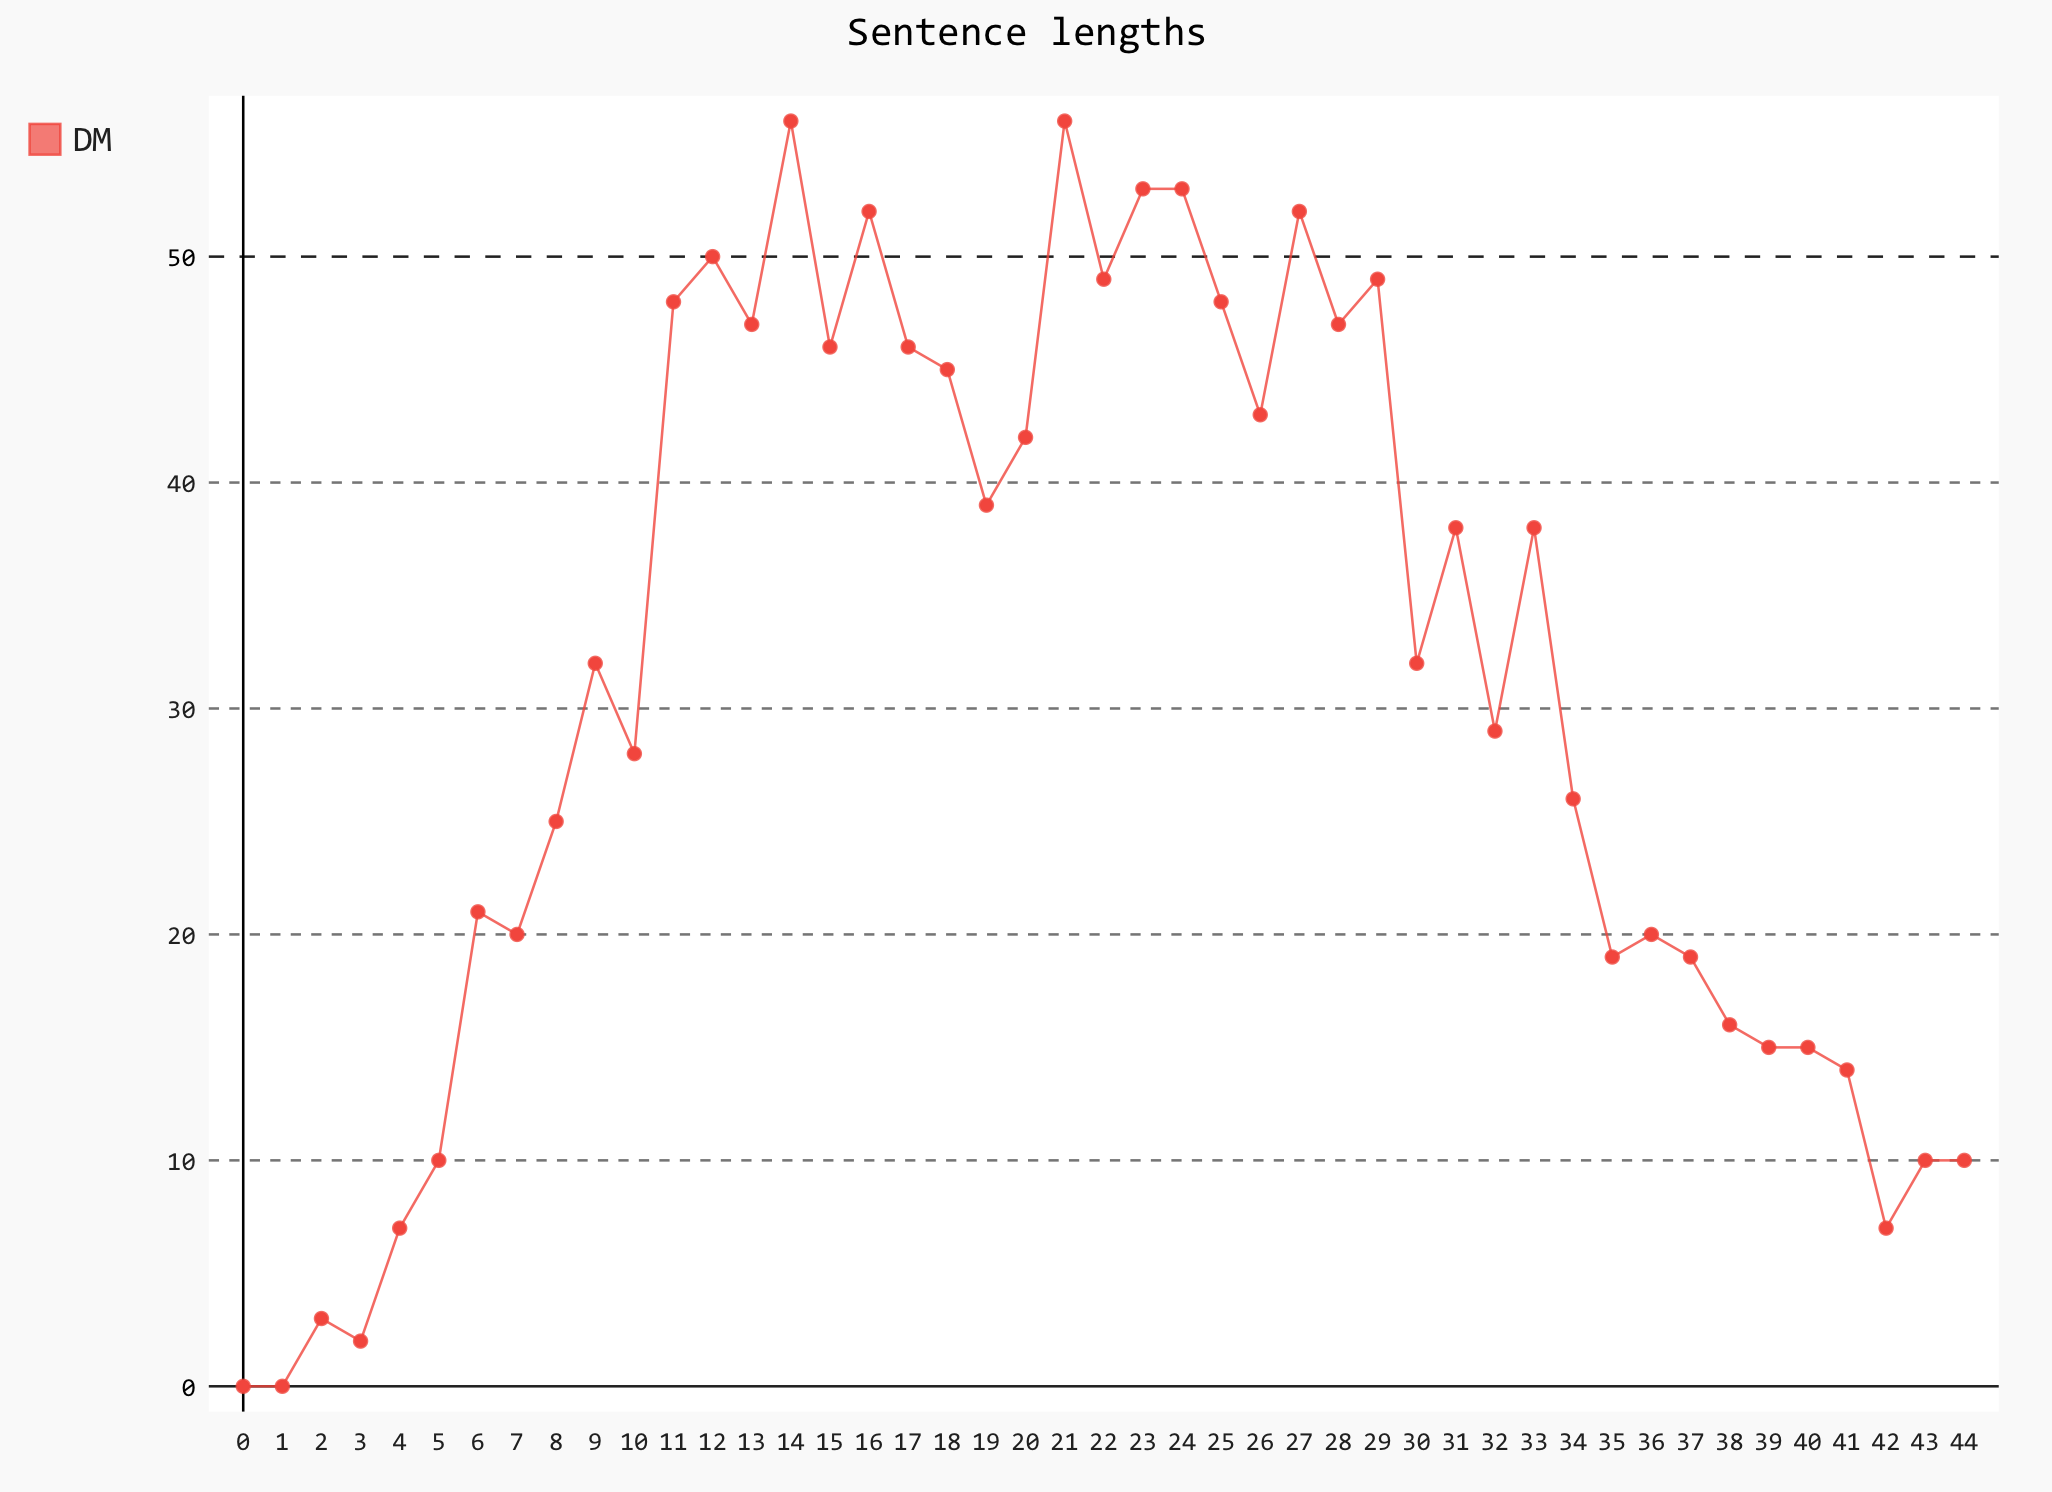
\includegraphics[width=\textwidth]{sentence_length}
% \label{fig:sentence_length}
% \end{figure}


\chapter{Experiments - Predicting Semantic Frames}
\label{chap:experiments}

% Keras with Tensorflow
% Recurrent nerual net (RNN) for training and predication. Used for solving many NLP tasks.

In this chapter we will present our own pipeline for predicting semantic frames. 
\chapter{Conclusion}
\label{chap:conclusion}

\backmatter
\bibliographystyle{apacite}
\bibliography{bib}

\end{document}
